Case study này sử dụng một video lớp học thật dài khoảng 18 phút 20 giây để minh họa toàn bộ quy trình CausClass, từ phát hiện hành vi đến báo cáo quan sát. Đây là phần trình diễn toàn trình, không phải bộ kiểm thử có đồ thị chuẩn. Bộ phát hiện chạy trên video, kết quả được ByteTrack theo dõi, gom vào các time bin 4 giây để tạo thành 276 bin chuỗi thời gian, sau đó đưa qua tìm kiếm AERCA có hướng dẫn bởi LLM và cuối cùng được kết xuất thành báo cáo quan sát dựa trên bằng chứng.

\begin{table}[htbp]
\centering
\caption{Thông tin case study video lớp học thật.}
\label{tab:case-study-video-info}
\begin{tabular}{lr}
\toprule
\textbf{Thuộc tính} & \textbf{Giá trị} \\
\midrule
Thời lượng video & khoảng 18 phút 20 giây \\
Độ dài time bin & 4 giây \\
Số bin chuỗi thời gian & 276 \\
Ngưỡng confidence & 0.1 \\
Ngưỡng IoU & 0.4 \\
Kích thước ảnh suy luận & 640 \\
YOLO batch size & 30 \\
Tracking patience & 2 giây \\
\bottomrule
\end{tabular}
\end{table}

Quy trình giữ nguyên tên lớp của bộ phát hiện khi mô hình đã dùng danh sách nhãn sạch \textit{Read}, \textit{Write}, \textit{Phone}, \textit{Bow}, \textit{Lean} và \textit{Talk}, không ánh xạ lại nhãn ở bước hậu xử lý. Các khung kiểm tra được lưu định kỳ để hỗ trợ đối chiếu thủ công: người đọc có thể so sánh chuỗi thời gian và báo cáo với hành vi nhìn thấy trong ảnh.

\begin{figure}[htbp]
  \centering
  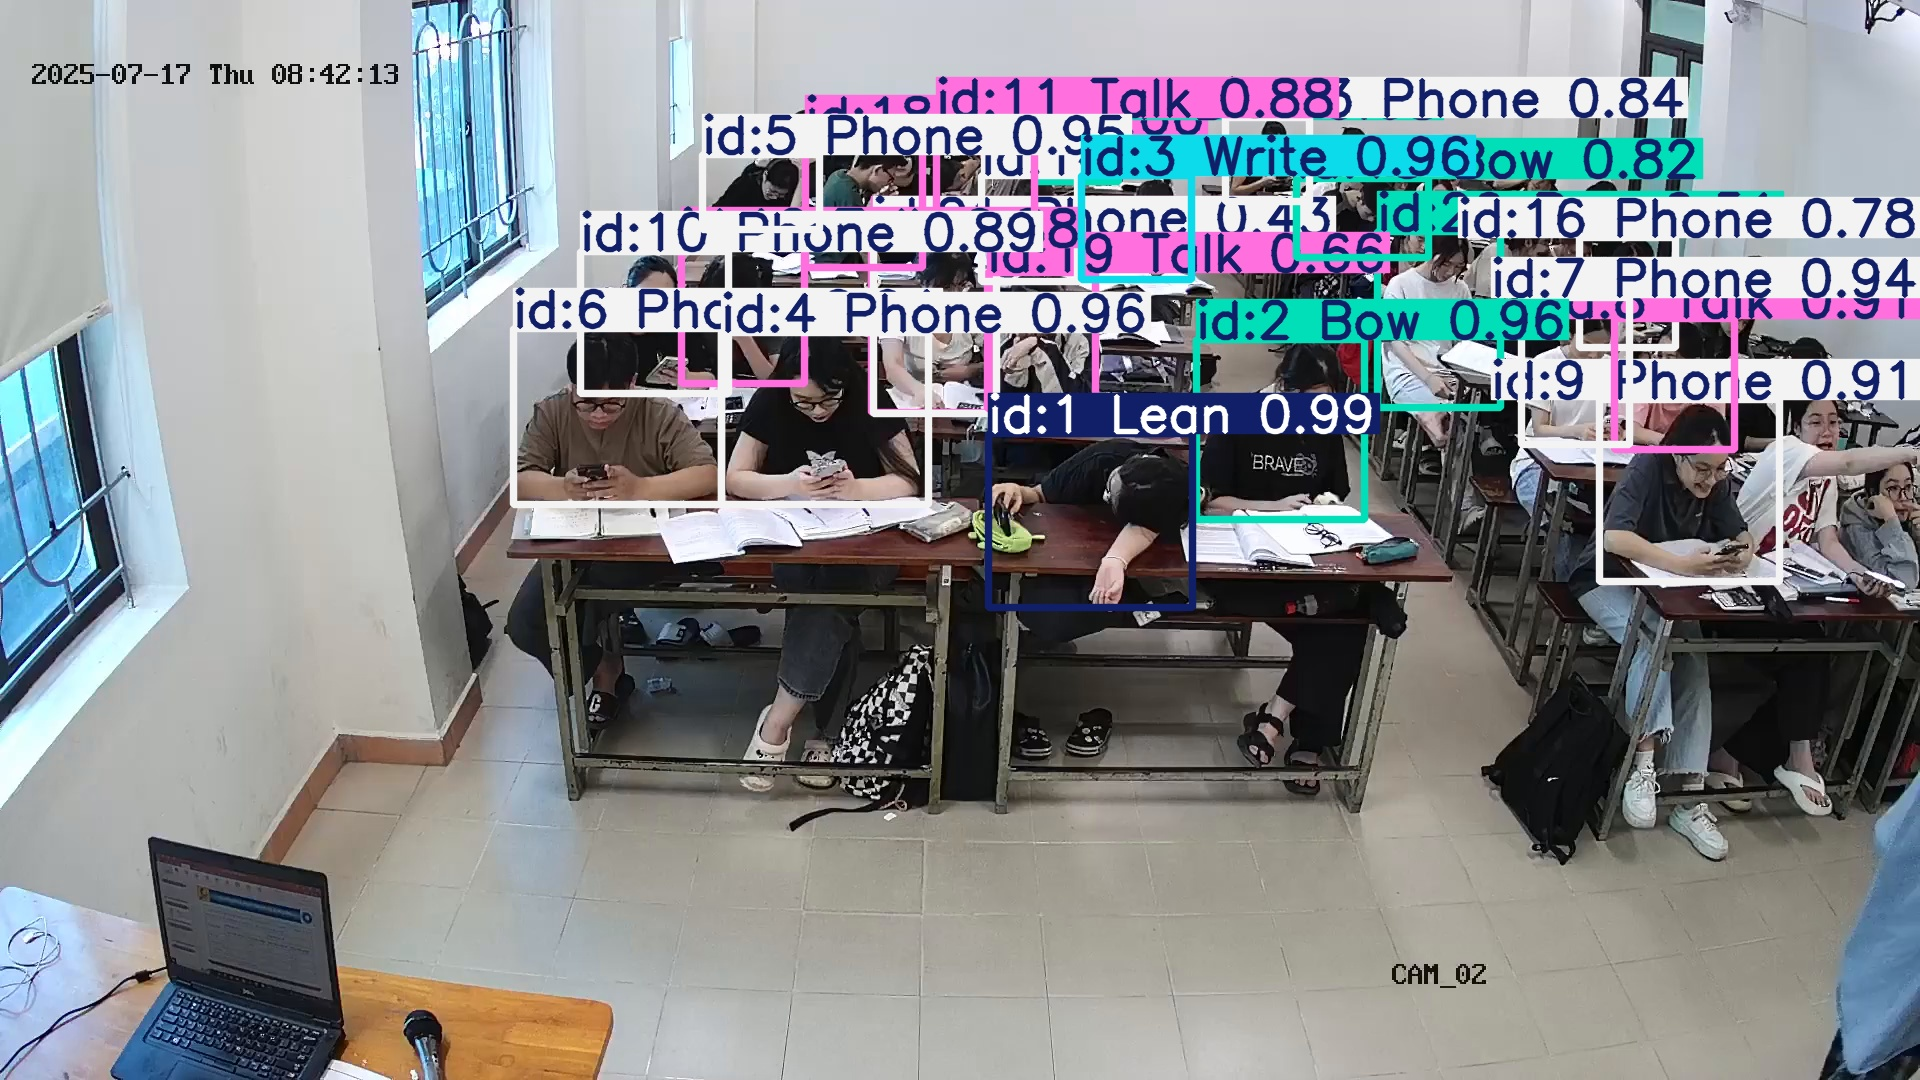
\includegraphics[width=0.7\textwidth]{figures/debug_frames/frame_00000000.jpg}
  \caption{Khung kiểm tra đại diện từ video thật tại frame 0.}
  \label{fig:case-study-debug-frame-0}
\end{figure}

\begin{figure}[htbp]
  \centering
  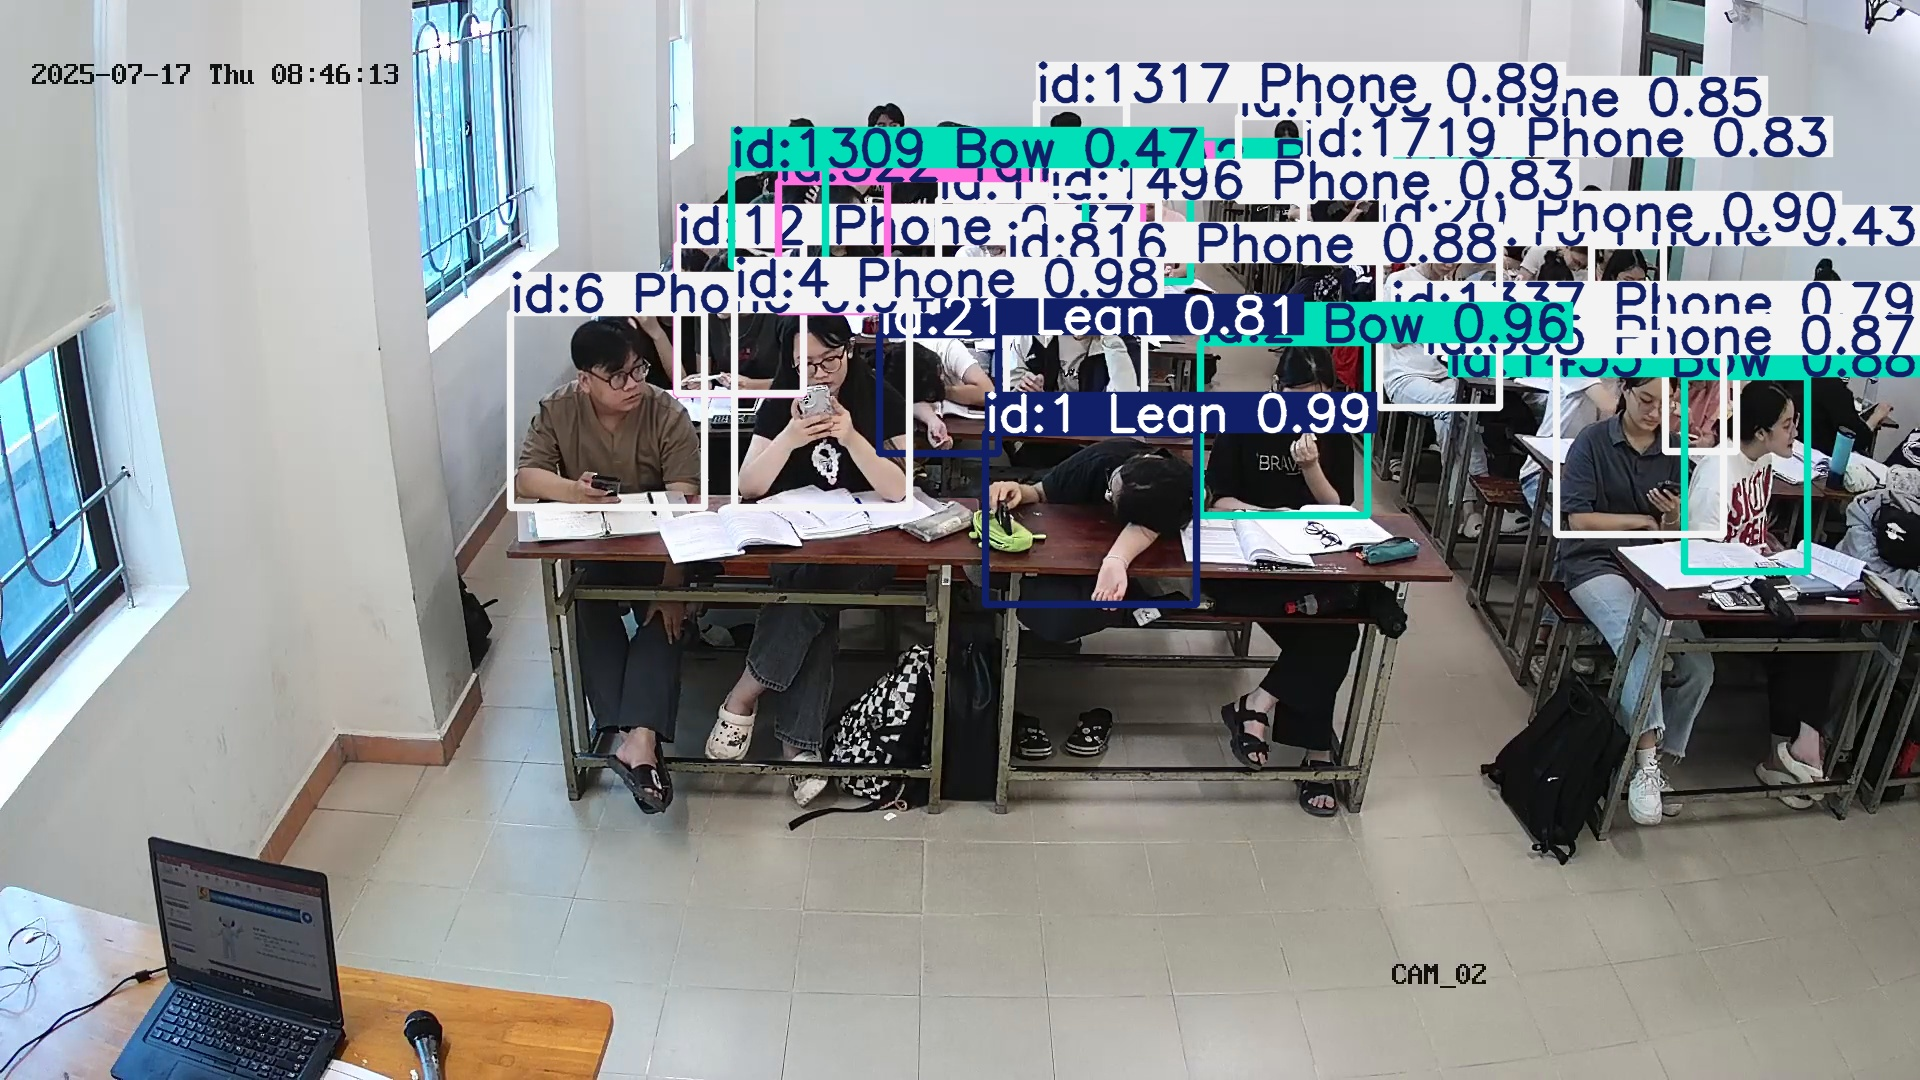
\includegraphics[width=0.7\textwidth]{figures/debug_frames/frame_00006000.jpg}
  \caption{Khung kiểm tra đại diện từ video thật tại frame 6000.}
  \label{fig:case-study-debug-frame-6000}
\end{figure}

\begin{figure}[htbp]
  \centering
  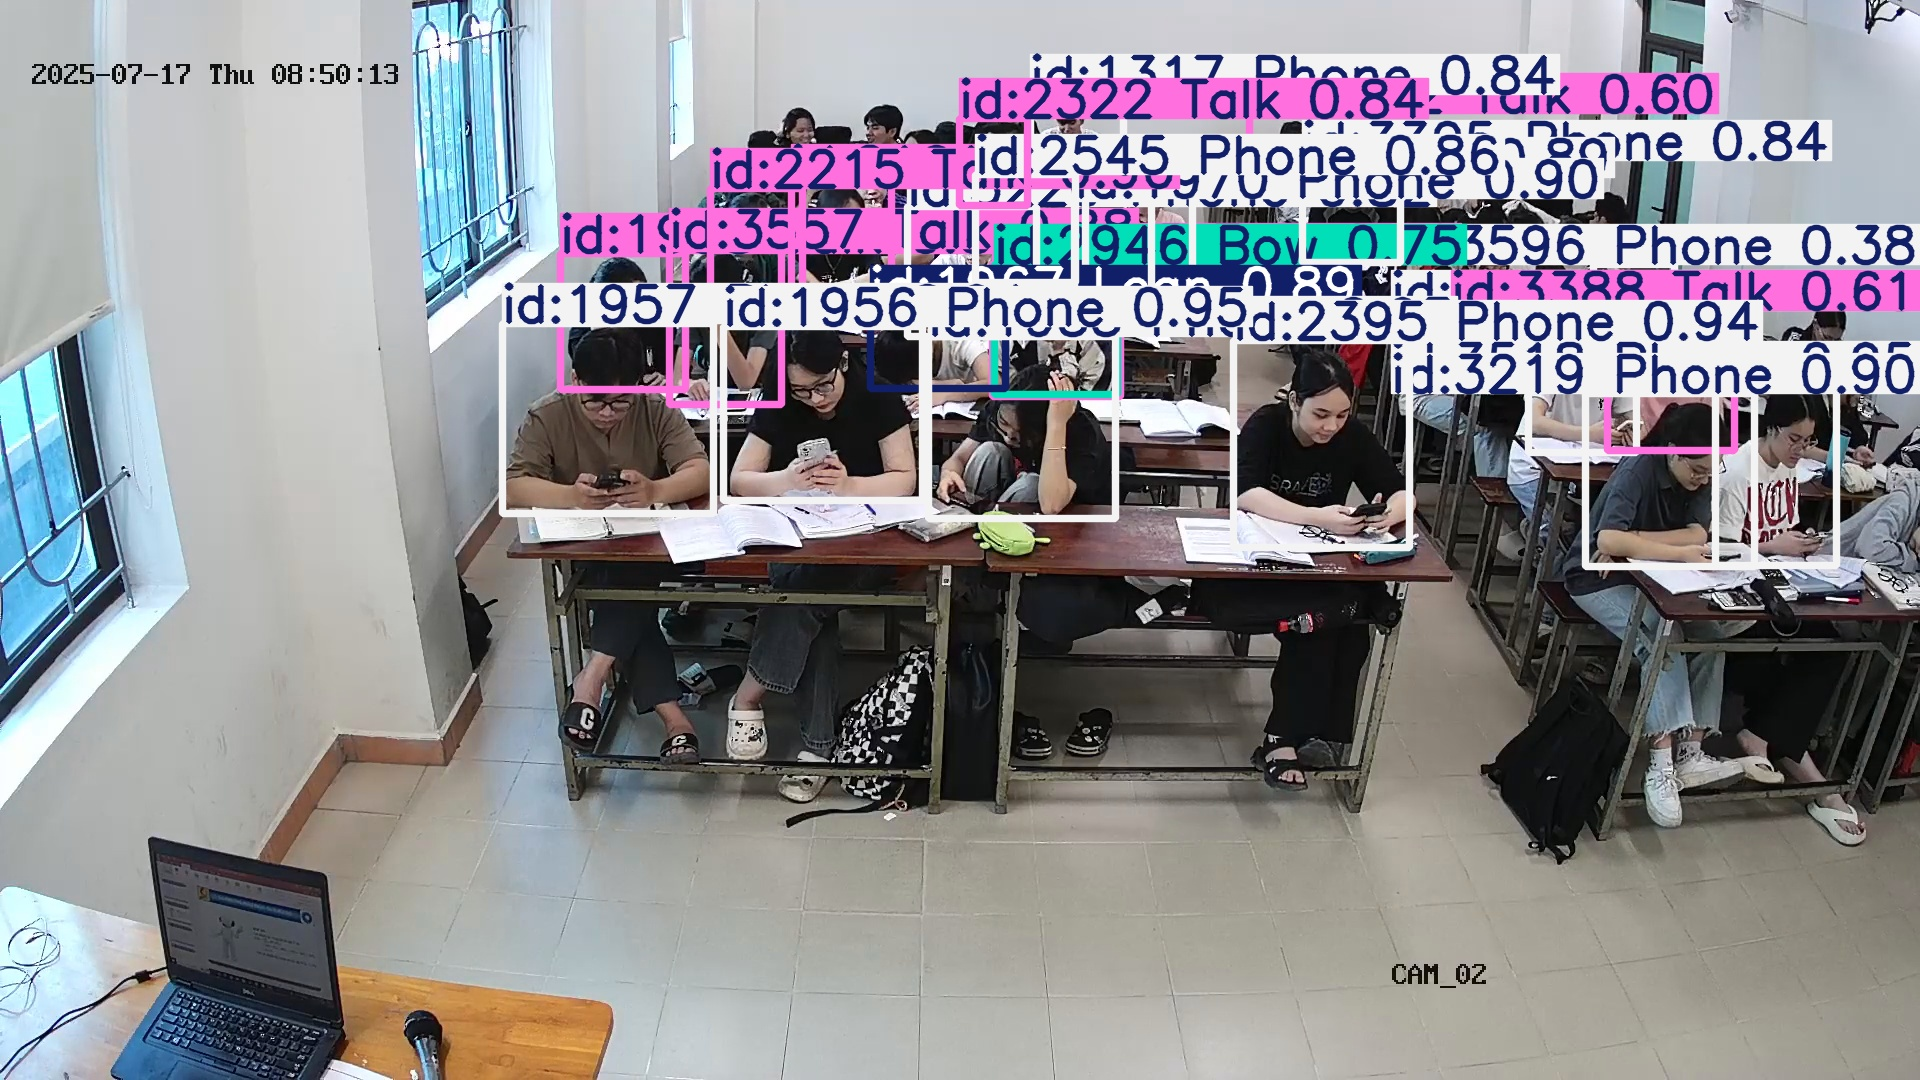
\includegraphics[width=0.7\textwidth]{figures/debug_frames/frame_00012000.jpg}
  \caption{Khung kiểm tra đại diện từ video thật tại frame 12000.}
  \label{fig:case-study-debug-frame-12000}
\end{figure}

\begin{table}[htbp]
\centering
\caption{Các đầu ra chính của case study.}
\label{tab:case-study-outputs}
\resizebox{\linewidth}{!}{%
\begin{tabular}{ll}
\toprule
\textbf{Nhóm đầu ra} & \textbf{Nội dung} \\
\midrule
Phát hiện & Danh sách sự kiện hành vi vi mô và khung kiểm tra \\
Chuỗi thời gian & CSV tỉ lệ hành vi theo 276 bin và siêu dữ liệu video \\
Đồ thị & Danh sách cạnh, ma trận kề, hình đồ thị và biểu đồ chuỗi thời gian \\
Báo cáo & Tóm tắt theo nguyên tắc nêu bằng chứng trước, dựa trên thống kê và cạnh đã kiểm chứng \\
\bottomrule
\end{tabular}
}
\end{table}

Đối với video thật, hệ thống sử dụng cùng logic beam search nhưng không tính Precision, Recall và F1 vì không có đồ thị chuẩn. Hệ số phạt cạnh kiểu BIC được đặt xấp xỉ \(\lambda=22\), được tỉ lệ hóa từ \(\lambda_{syn}=65\) của thực nghiệm tổng hợp theo độ dài chuỗi:
\begin{equation}
\label{eq:real-lambda-scaling}
    \lambda_{real}=\lambda_{syn}\frac{n_{real}}{n_{syn}}\frac{\log n_{syn}}{\log n_{real}}.
\end{equation}
Với \(n_{syn}=1000\) và \(n_{real}=276\), công thức cho giá trị xấp xỉ 22.06; quy trình dùng \(\lambda=22\) như một thiết lập thăm dò cho chuỗi thật ngắn hơn.

Trước khi sinh báo cáo, CausClass tạo hai nhóm bằng chứng đầu vào: thống kê mô tả của từng hành vi và các xu hướng biến đổi theo thời gian. Bảng~\ref{tab:case-study-descriptive-stats} tóm tắt nhóm bằng chứng thứ nhất. Các giá trị là phần trăm sự kiện hành vi được bộ phát hiện ghi nhận trong từng time bin, không phải phần trăm chính xác của toàn bộ học sinh trong lớp.

\begin{table}[htbp]
\centering
\caption{Thống kê mô tả hành vi trong case study.}
\label{tab:case-study-descriptive-stats}
\begin{tabular}{lrrrr}
\toprule
\textbf{Hành vi} & \textbf{Tỉ lệ TB} & \textbf{Cực đại} & \textbf{Độ lệch chuẩn} & \textbf{Tỉ lệ bin hoạt động} \\
\midrule
Phone & 40.624\% & 65.62\% & 13.444\% & 100.000\% \\
Talk & 28.345\% & 52.05\% & 9.967\% & 100.000\% \\
Bow & 18.789\% & 41.07\% & 8.772\% & 99.638\% \\
Read & 5.872\% & 37.33\% & 10.183\% & 29.348\% \\
Write & 3.843\% & 32.14\% & 6.886\% & 39.493\% \\
Lean & 2.527\% & 14.29\% & 2.786\% & 65.580\% \\
\bottomrule
\end{tabular}
\end{table}

Nhóm bằng chứng thứ hai là xu hướng theo thời gian. \textit{Phone} giảm dần với hệ số tuyến tính khoảng \(-0.100\) điểm phần trăm mỗi bin, trong khi \textit{Read} và \textit{Write} tăng lần lượt khoảng 0.091 và 0.049 điểm phần trăm mỗi bin. \textit{Bow} tăng nhẹ khoảng 0.020 điểm phần trăm mỗi bin, còn \textit{Lean} và \textit{Talk} giảm lần lượt khoảng \(-0.024\) và \(-0.036\) điểm phần trăm mỗi bin. Nếu chia video thành ba phần bằng nhau, \textit{Phone} vẫn là hành vi trội nhất ở cả ba phần, với trung bình 45.903\%, 46.863\% và 29.105\%. Ở phần cuối, \textit{Read} tăng lên 17.292\% và \textit{Write} tăng lên 10.096\%, trong khi \textit{Talk} giảm từ 36.838\% ở phần giữa xuống 20.987\%. Những lát cắt này chỉ là chia đoạn kỹ thuật của video, không nhất thiết tương ứng với các pha sư phạm của tiết học.

Từ các thống kê mô tả, xu hướng thời gian và danh sách cạnh đã kiểm chứng, hệ thống sinh báo cáo quan sát theo nguyên tắc nêu bằng chứng trước. Trong thiết lập triển khai, mô hình báo cáo là \textit{DeepSeek-v4-Pro}; mô hình nhận tóm tắt chuỗi thời gian và danh sách cạnh, sau đó trả về báo cáo JSON. Bộ kết xuất xác định chỉ trình bày lại các thông tin đã có trong đầu vào, nhờ đó tránh việc mô hình ngôn ngữ đổi tên cạnh, thêm cạnh mới hoặc diễn giải vượt quá bằng chứng.

Phần dưới đây là báo cáo quan sát được đưa vào case study. Báo cáo được biên tập theo hướng gọn hơn bản sinh ban đầu: các mục trùng nhau về diễn biến hành vi được gộp lại, các số liệu đã có trong bảng không bị lặp nguyên văn, còn các nhận xét quan trọng nhất được giữ để người quan sát biết nên kiểm tra đoạn video nào.

\subsection{Báo cáo quan sát}

\paragraph{Diễn biến chính.}
\textit{Phone} là hành vi chiếm ưu thế trong phiên quan sát, với tỉ lệ trung bình 40,6\% và cực đại 65,6\%, nhưng xu hướng chung giảm dần theo thời gian. \textit{Talk} và \textit{Bow} xuất hiện ổn định trong hầu hết các khoảng thời gian; \textit{Talk} đạt mức cao nhất ở giai đoạn giữa rồi giảm, còn \textit{Bow} tăng nhẹ. \textit{Read} và \textit{Write} nhìn chung ít xuất hiện hơn nhưng tăng rõ rệt trong một phần ba cuối phiên. \textit{Lean} là hành vi tương đối hiếm và có xu hướng giảm nhẹ.

\paragraph{Liên kết thời gian được phát hiện.}
Đồ thị cuối cùng gồm ba cạnh: \textit{Talk}\(\rightarrow\)\textit{Phone}, \textit{Talk}\(\rightarrow\)\textit{Read} và \textit{Phone}\(\rightarrow\)\textit{Read}. Trong đó, \textit{Talk}\(\rightarrow\)\textit{Phone} là liên kết dương mạnh nhất; \textit{Talk}\(\rightarrow\)\textit{Read} là liên kết dương yếu; còn \textit{Phone}\(\rightarrow\)\textit{Read} là liên kết âm yếu, gợi ý khả năng tồn tại sự đánh đổi giữa hai tín hiệu hành vi trong chuỗi quan sát.

\paragraph{Diễn giải có điều kiện.}
Mức \textit{Phone} cao có thể đi kèm với mức \textit{Read} thấp hơn ở thời điểm sau, nhưng nhận xét này chỉ là giả thuyết dựa trên liên kết thời gian. Liên kết giữa \textit{Talk} và \textit{Read} có thể xuất hiện trong các hoạt động hợp tác hoặc đọc thành tiếng, trong khi liên kết \textit{Talk}\(\rightarrow\)\textit{Phone} có thể phản ánh tương tác xã hội liên quan đến việc sử dụng điện thoại. Các cách diễn giải này cần được kiểm tra bằng video gốc, vì mô hình không quan sát được mục tiêu bài học, chỉ dẫn của giáo viên hoặc bối cảnh ngoài khung hình.

\paragraph{Điểm cần kiểm tra thủ công.}
Người quan sát nên xem lại các thời điểm \textit{Read} tăng mạnh để bảo đảm chúng không bị nhầm với tư thế \textit{Bow}; kiểm tra các bin mà \textit{Phone} đạt đỉnh để loại trừ khả năng phát hiện sai; xem lại các khoảng thời gian \textit{Write} gần như biến mất; và đối chiếu đoạn cuối phiên, nơi \textit{Read} và \textit{Write} tăng đột ngột. Những bước kiểm tra này giúp biến báo cáo tự động thành danh sách gợi ý kiểm chứng, thay vì kết luận sư phạm cuối cùng.

\subsection{Giao diện web phân tích trực quan}

Bên cạnh các tệp kết quả dạng bảng, đồ thị và báo cáo văn bản, case study còn được trình bày qua một giao diện web nhằm hỗ trợ quan sát trực quan toàn bộ quy trình phân tích. Giao diện này không thay đổi thuật toán phát hiện hay tìm kiếm đồ thị, mà đóng vai trò lớp tổng hợp kết quả để người dùng kiểm tra nhanh video đầu vào, thông số phân tích, thống kê mô tả, đồ thị liên kết thời gian, báo cáo quan sát và diễn biến các hành vi theo thời gian trong cùng một màn hình.

Hình~\ref{fig:web-visual-analysis-demo} minh họa bản demo của giao diện với video lớp học thật đã dùng trong case study. Phần đầu trang hiển thị thông tin video và số lượng time bin; cột trái tóm tắt thống kê mô tả và đồ thị thời gian; vùng giữa trình bày báo cáo quan sát theo các câu hỏi chính; còn cột phải trực quan hóa chuỗi thời gian của các hành vi. Cách bố trí này giúp người quan sát chuyển từ số liệu tổng hợp sang kiểm tra xu hướng cụ thể mà không phải mở riêng từng tệp đầu ra.

\begin{figure}[htbp]
  \centering
  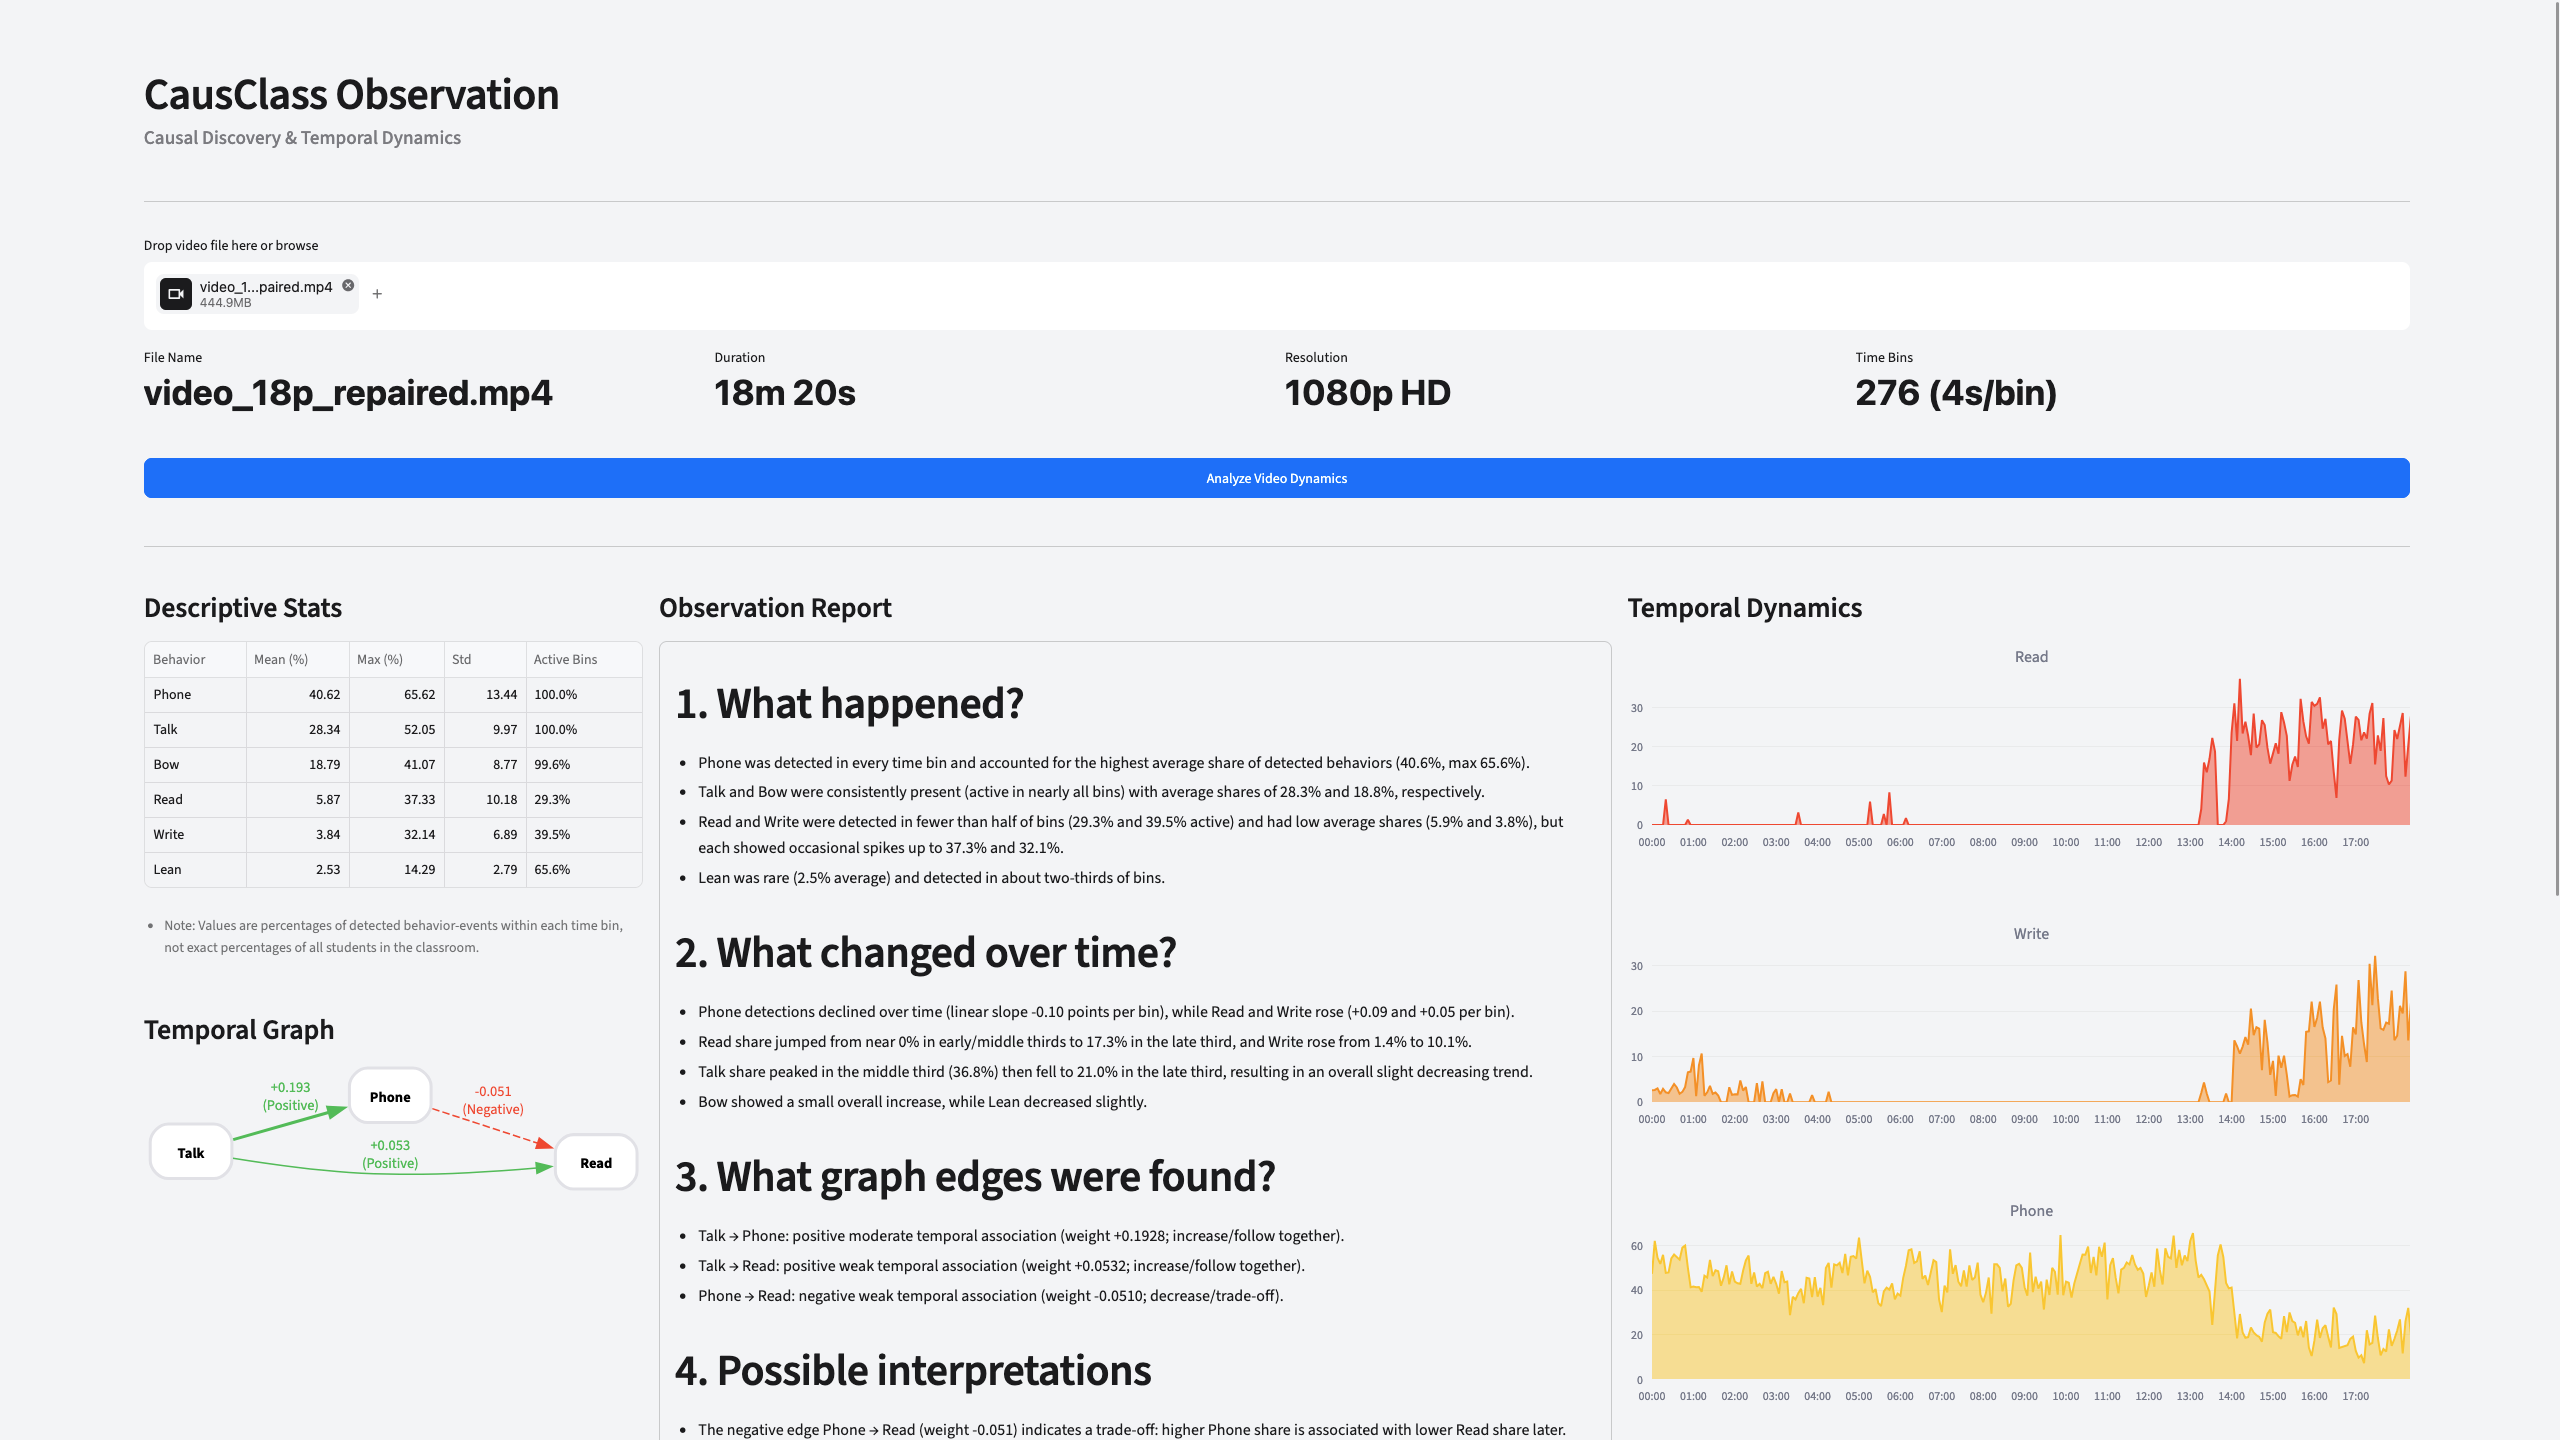
\includegraphics[width=\linewidth]{figures/web_visual_analysis_demo.png}
  \caption{Giao diện web demo dùng để phân tích trực quan kết quả case study CausClass.}
  \label{fig:web-visual-analysis-demo}
\end{figure}

Do giao diện chỉ hiển thị lại các kết quả đã được sinh từ pipeline, các biểu đồ và nhận xét trong màn hình vẫn cần được đọc theo cùng nguyên tắc thận trọng như báo cáo văn bản: chúng là bằng chứng quan sát được từ bộ phát hiện và chuỗi thời gian, không phải kết luận trực tiếp về nguyên nhân sư phạm. Tuy vậy, việc đặt bảng thống kê, đồ thị và báo cáo cạnh nhau giúp rút ngắn bước kiểm chứng thủ công, đặc biệt khi cần tìm nhanh các đoạn video có biến động mạnh hoặc các cạnh thời gian cần xem lại.

Tóm lại, case study cho thấy quy trình có thể vận hành từ video đầu vào đến báo cáo cuối cùng, đồng thời có thể được đóng gói thành giao diện trực quan để hỗ trợ kiểm tra kết quả. Nó cũng nhấn mạnh giới hạn của hệ thống: tỉ lệ phát hiện không phải tỉ lệ học sinh, các đoạn bằng nhau của video không nhất thiết là pha bài học, trọng số cạnh không phải kiểm định thống kê, và đồ thị không phải phán quyết về hành vi học sinh.